\documentclass{beamer}

\usepackage[utf8]{inputenc}
\usecolortheme{beaver}
\usepackage{caption}
\usepackage{subcaption}
\usepackage{mathtools}
\usepackage{todonotes}
\usepackage{amsmath}
\usepackage{bm}
\usepackage{listings}
\usepackage{ragged2e}
\usepackage{titlecaps}
\usepackage{fancyvrb}

\def\ci{\perp\!\!\!\!\!\perp}

\newtheorem{proposition}{Proposition}
\Addlcwords{for a is but and with of in as the etc on to if}

\setbeamertemplate{section in toc}{\inserttocsectionnumber.~\inserttocsection}
\usetheme{Boadilla}
\makeatletter
\setbeamertemplate{footline}{%
    \leavevmode%
    \hbox{%
        \begin{beamercolorbox}[wd=.3\paperwidth,ht=2.25ex,dp=1ex,center]{author in head/foot}%
            \usebeamerfont{author in head/foot}\insertshortauthor\expandafter\beamer@ifempty\expandafter{\beamer@shortinstitute}{}{~~(\insertshortinstitute)}
        \end{beamercolorbox}%
        \begin{beamercolorbox}[wd=.55\paperwidth,ht=2.25ex,dp=1ex,center]{title in head/foot}%
            \usebeamerfont{title in head/foot}\insertshorttitle
        \end{beamercolorbox}%
        \begin{beamercolorbox}[wd=.15\paperwidth,ht=2.25ex,dp=1ex,right]{date in head/foot}%
            \usebeamerfont{date in head/foot}\insertshortdate{}\hspace*{2em}
            \insertframenumber{} / \inserttotalframenumber\hspace*{2ex} 
        \end{beamercolorbox}}%
        \vskip0pt%
    }
\makeatother

\begin{document}

\title[]{Introduction to Casual Inference using pgmpy}
\author{Ankur Ankan}
\institute{Radboud University}
\date{}

\maketitle

\begin{frame}{Predictive Models vs Causal Questions}
\end{frame}

\begin{frame}{Motivating Examples}
	\begin{itemize}
		\item Finding how variables interact.
		\item Key drivers of an outcome.
		\item Feature Selection
	\end{itemize}
\end{frame}

\begin{frame}{Two Main Framworks}
	Mathematical formulations of causal inference:
	\begin{itemize}
		\item Potential Outcomes Framework (aka Rubin's Casual Model)
			\begin{itemize}
				\item Counterfactual is at the center.
				\item Provides methods to robustly estimate the counterfactual given assumptions are satisfied.
				\item Flexible methods that can give estimates even when some of the assumptions fail.
			\end{itemize}
		\item Directed Acyclic Graphs (DAG) / Structural Equation Models (SEMs)
			\begin{itemize}
				\item The causal diagram (DAG) is at the center.
				\item Using the DAG, we can define estimators of interest.
				\item Assumptions of model are more explicit.
			\end{itemize}
	\end{itemize}
\end{frame}

\begin{frame}{Landscape of Causal Inference Python Packages}
	\begin{itemize}
		\item Potential Outcomes Framework (aka Rubin's Causal Model)
			\begin{itemize}
				\item Propensity score methods
					\begin{figure}
						\includegraphics[scale=0.1]{imgs/dowhy.png}
					\end{figure}
				\item Doubly Robust Estimation
					\begin{figure}
						\includegraphics[scale=0.1]{imgs/doubleml.png}
					\end{figure}
				\item Meta Learners: T-Learner, S-Learner, X-Learner.
					\begin{figure}
						\includegraphics[scale=0.1]{imgs/causalml.png}
					\end{figure}
			\end{itemize}
		\item Directed Acyclic Graphs / Structural Causal Models: 
			\item pgmpy
				\begin{figure}
					\includegraphics[scale=0.1]{imgs/pgmpy.png}
				\end{figure}
			\item casualnex
				\begin{figure}
					\includegrap
				\end{figure}
	\end{itemize}
\end{frame}

\begin{frame}{A General Workflow in the DAG Framework}

\begin{figure}[t]
	\centering
	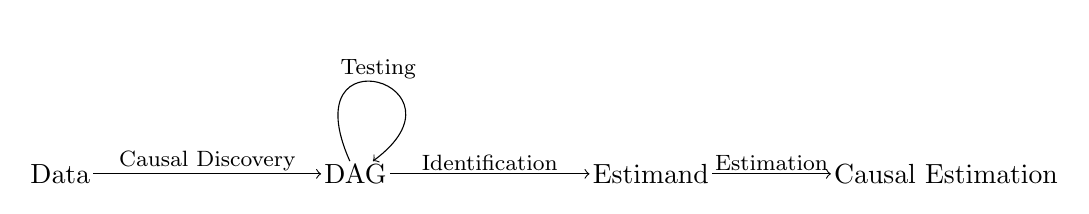
\begin{tikzpicture}[yscale=1, xscale=0.75, inner sep=1pt]
	\tikzstyle{every node}=[align=left]
		\node (data) at (0, 0) {Data};
		\node (dag) at (5, 0) {DAG};
		\node (estimand) at (10, 0) {Estimand};
		\node (estimation) at (15, 0) {Causal Estimation};

		\draw[->] (data) to node[midway, above]{\footnotesize Causal Discovery} (dag);
		\draw[->] (dag) to node[midway, above] {\footnotesize Identification} (estimand);
		\draw[->] (estimand) to node[midway, above] {\footnotesize Estimation} (estimation);
		\draw[->] (dag) [out=120, in=30, looseness=10] to node[midway, above] {\footnotesize Testing} (dag);
	\end{tikzpicture}
	\label{fig:workflow}
\end{figure}

\end{frame}

\begin{frame}{What does pgmpy provide}
\end{frame}

\begin{frame}{Causal Discovery}
	\begin{figure}[t]
		\centering
		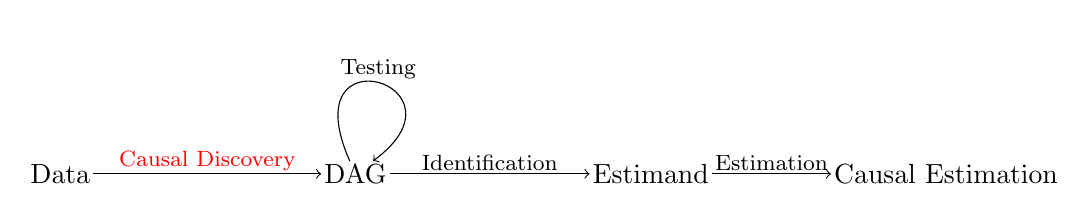
\begin{tikzpicture}[yscale=1, xscale=0.75, inner sep=1pt]
		\tikzstyle{every node}=[align=left]
			\node (data) at (0, 0) {Data};
			\node (dag) at (5, 0) {DAG};
			\node (estimand) at (10, 0) {Estimand};
			\node (estimation) at (15, 0) {Causal Estimation};
	
			\draw[->] (data) to node[midway, above]{\footnotesize \textcolor{red}{Causal Discovery}} (dag);
			\draw[->] (dag) to node[midway, above] {\footnotesize Identification} (estimand);
			\draw[->] (estimand) to node[midway, above] {\footnotesize Estimation} (estimation);
			\draw[->] (dag) [out=120, in=30, looseness=10] to node[midway, above] {\footnotesize Testing} (dag);
		\end{tikzpicture}
		\label{fig:workflow}
	\end{figure}

	\begin{itemize}
		\item Given a dataset learn the network structure.
		\item The most challenging step of using the DAG framework.
	\end{itemize}
\end{frame}

\begin{frame}{PC algorithm}
	Constraint-Based Algorithm: Exploits Conditional Indpendences in the data to construct the DAG.
\end{frame}

\begin{frame}{Hill-Climb Search}
	Score based: Tries to optimize the score by doing local changes.
\end{frame}

\begin{frame}{And it continues}
\end{frame}

\begin{frame}{Casual Discovery}
	Learnt models are usually incorrect.
	\begin{itemize}
		\item Really have to remember that: "All models are wrong, but some are useful" - George Box
		\item Many automated algorithms but most of them would make mistakes.
		\item Usually need to have some manual intervention. Need tools to guide this intervention.
		\item As the ground truth is not known, difficult to test how good our model is. Adhoc methods to help with it.
	\end{itemize}
	How do we improve on these methods?
	We have implemented a bunch of method to help users create these models
\end{frame}

\begin{frame}{Expert Knowledge Integration}
	Specify blacklisted and whitelisted edges.
\end{frame}

\begin{frame}{Expert Knowledge} 
	Specify initial model.
\end{frame}

\begin{frame}
	Specify fixed edges.
\end{frame}

\begin{frame}{Model evaluation}
	Lots of options for learning the models. How do know which one is the best?
	\begin{itemize}
		\item Implied CIs: Benefits, local testing, gives a hint of where things are wrong.
		\item Fisher C: Similar to implied CIs but summerizes the whole model fit.
		\item Compare models using likelihood or a scoring metric to see which fits better.
	\end{itemize}
\end{frame}

\begin{frame}{Causal Discovery Algorithms learn a CPDAG}
	\begin{itemize}
		\item Trying to learn a network structure which matches the covariance
			structure.
		\item Multiple networks can represent the same casual structure.
		\item Structure learning algorithms usually a DAG.
	\end{itemize}

	Pairwise edge orientation rules.
\end{frame}

\begin{frame}{Minimal Orientation}
\end{frame}

\begin{frame}{LLM Based Structure Learning}
\end{frame}

\begin{frame}{Using DAG in the PO framework}
	As DAGs explicitly show all the information, it can be used to make
	decisions in the PO framework as well.

	The graph can be put into pywhy as well.
\end{frame}

\begin{frame}{Identification}
	\begin{itemize}
		\item Second step: Assuming that we have an oriented DAG.
		\item Everything is identified in the case of fully observed models.

		\item When latent variables are present, need to determine identfiablity.
	\end{itemize}
\end{frame}

\begin{frame}{do-calculus}
	\begin{itemize}
		\item Rules of do-calculus provide a full solution but no
			efficient algorithm.
		\item Other criterion with efficient algorithm but can only
			identify special cases.
		\item Back-door criterion
		\item Front-door criterion
		\item Instrumental variables.
	\end{itemize}
\end{frame}

\begin{frame}{Backdoor Criterion}
\end{frame}

\begin{frame}{Front-door Criterion}
\end{frame}

\begin{frame}{Instrumental Variables}
\end{frame}

\begin{frame}{pgmpy takes care of all this}
\end{frame}

\begin{frame}{Estimation}
	\begin{itemize}
		\item The identification method give the estimand.
		\item Use your favourite method for actual estimation.
	\end{itemize}
\end{frame}

\begin{frame}{Simulations}
\end{frame}

\begin{frame}{Extensibiilty}
	Lots of new methods are being developed.
	Easy to integrate new algorithms.
\end{frame}

\begin{frame}{Lot more functionality}
	\begin{itemize}
		\item Other models such as SEM, Dynamic Bayesian Networks, Cluster Graphs.
		\item Probabilistic Inference
		\item Approximate Inference using Sampling
		\item Reading writing to interface with other packages.
		\item Plotting functionality
		\item Parameter Estimation
	\end{itemize}
\end{frame}

\begin{frame}{Conclusion}
	\begin{itemize}
		\item Building causal models is an iterative process.
		\item Integrating expert knowledge can help a lot.
		\item Things are easy once we have the graph.
	\end{itemize}
\end{frame}

\begin{frame}{Future Plans}
	\begin{itemize}
		\item Focus on developing more practical methods.
		\item Wider support for mixed data.
	\end{itemize}
\end{frame}

\begin{frame}
	Thank you.

	Consulting Company: Squanch Labs. Feel free to reach out to discuss use cases etc.
\end{frame}

\begin{frame}{Extra slide}
	When to use PO vs DAG framework?
\end{frame}

\begin{frame}
	How does it compare to Shapley values 
	\begin{itemize}
		\item Still prediction based. Does not matter if perturbing direct effect variable or undirect.
		\item Can show an example where Shapley values would still find an association, but causal inference would not. The standard confounding case.
	\end{itemize}
\end{frame}
\end{document}
